\chapter{Implementacja}
\thispagestyle{chapterBeginStyle}

\section{Opis komponentów i ich połączeń}
    W programie implementującycm algorytm będący obiektem badań można wyróżnić 3 główne komponenty:
    \begin{itemize}
        \item \textbf{Algorytm} zaimplementowany w języku programowania \textbf{PROLOG}
        \item \textbf{Generator grafów} zaimplementowany w formie modułu w języku programowania \textbf{Python}
        \item \textbf{Warstwa graficzna} (GUI) zaimplementowana w języku programowania \textbf{Python} przy użyciu bibloteki \textbf{Tkinter}
    \end{itemize}
    Naistostniejszą z perspektywy użytkownika jest \textbf{Warstwa graficzna}. Jest to program, którego uruchomienie pozwala na 
    interakcję z utworzonym narzędziem w przyjazny dla użytkownika sposób. Istnieje również możliwość uruchomienia algorytmu z pominięciem 
    warstwy graficznej, o czym można dowiedzieć się więcej w sekcji \ref{CommandLine}.
    Z wyświetlonego menu użytkownik może wybrać przykładowe, wcześniej spreparowane światy, zdefiniować swój stan początkowy oraz cel (w niektórych 
    światach cel jest intuicyjny, więc jego definicja nie jest od użytkownika wymagana) i uruchomić algorytm. Wynikiem działania programu jest 
    plan, który wyświetlony jest w formie tekstowej z opisem na kroki, oraz dwa grafy: graf pełen (zawierający wszystkie składowe opisane 
    w \ref{GRAPHPLANRozdzial}) oraz graf uproszczony, który zawiera jedynie niezbędne stany oraz akcje wymagane do zrozumienia wygenerowanego planu.
    Poniższy schemat klarownie przedstawia relacje między komponentami w trakcie działania programu:
    \begin{figure}[H]
        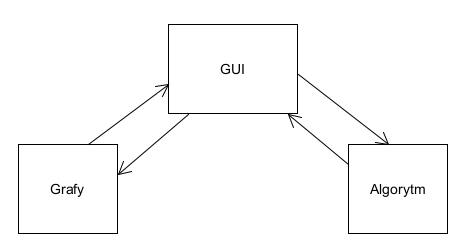
\includegraphics[scale=0.5]{zaleznosci}
        \centering
        \caption{Zależności między komponentami}
    \end{figure}
    Główna jednostką sterującą jest warstwa graficzna. W momencie naciśnięcia przez użytkownika odpowiedniego przycisku generującego rozwiązania, warstwa 
    graficzna zbiera wszystkie niezbędne informacje: w jakim świecie użytkownik pracuje, w jaki sposób zdefiniował warunki początkowe, oraz jakie cele 
    chce on uzyskać. Następnie obrobione informacje przesyłane są do algorytmu, który poza wygenerowaniem planu, do pliku tekstowego wypisuje 
    stany, akcje oraz mutexy dla każdej z warstw. Następnie algorytm przesyła swoją odpowiedź do GUI, 
    który wysyła żadanie wygenerowania grafów do odpowiednich komponentów odpowiedzialnych za ich 
    generowanie. W skład komponentu "Grafy" wchodzą dwie klasy, przy czym każda z nim generuje unikalny graf.

\section{Implementacja algorytmu}
    Algorytm \textbf{GRAPHPLAN} został zaimplementowany w języku programowania PROLOG. Poniższe diagramy przedstawiają proces  
    generowania pojedynczego planu.
    \begin{figure}[H]
        \label{PetlaGlowna}
        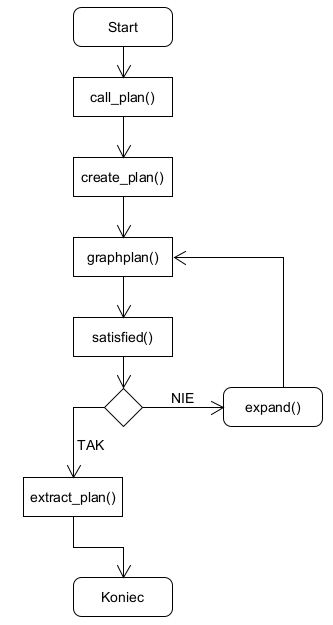
\includegraphics[scale=0.75]{GRAPHPLAN_petla_glowna}
        \centering
        \caption{Główna pętla algorytmu}
    \end{figure}

    \begin{definition}
        \label{Predykat}
        \textbf{Klauzula} -- przedstawiona informacja o świecie
    \end{definition}

    \begin{definition}
        \label{Fakt}
        \textbf{Fakt} -- informacja o świecie, która jest zawsze prawdziwa
    \end{definition}

    \begin{definition}
        \label{Regula}
        \textbf{Reguła} -- informacje, które są prawdziwe, po spełnieniu pewnych warunków
    \end{definition}

    \begin{definition}
        \label{Predykat}
        \textbf{Predykat} -- sposób wyrażania warunków w programowaniu w logice
    \end{definition}


    Przed rozpoczęciem omawiania struktury programu wprowadzono podstawowe definicje stosowane w programowaniu w logice. Przykładem klauzuli jest 
    zdanie $kobieta(anna).$ informujące program o tym, iż Anna jest kobietą. Ze względu na sposób reprezentacji danych w języku programowania PROLOG, 
    wszystkie stałe określane są małymi literami, gdyż ciągi znaków zaczynające się wielką literą zarezerwowane są dla \textit{zmiennych}. Należy 
    również zwrócić uwagę na wykorzystanie znaku przystankowego w postaci kropki (\textbf{.}), przedstawiający koniec przekazywanej informacji. 
    $kobieta(anna).$ również jest przykładem jednoargumentowego predykatu. Predykaty jednoargumentowe często określanę są mianem \textit{własności}.
    Predykaty o większej liczbie argumentów często nazywane są \textit{relacjami}. W Prologowej nomenklaturze predykaty zapisuję się zgodnie 
    z następującą strukturą: \textit{X/Y}, gdzie \textit{X} oznacza nazwę relacji (nagłówek), a \textit{Y} liczbę argumentów przyjmowaną przez 
    opisywany predykat. Zgodnie z powyższym zapis $kobieta/1$ oznacza, iż relacja kobieta przyjmuje jeden argument.
    Zdanie $kolor(brązowy).$ jest przykładem faktu, czyli zdania zawsze prawdziwego. Fakty różnią się od reguł tym, iż reguły nie muszą być zawsze prawdziwe.
    W sekcji \ref{DefinicjeSwiata} wprowadzono przykład reguły, wraz z opisem jej struktury. 

    Predykat o nazwie $call\_plan/2$ odpowiada za utworzenie pliku tekstowego (nazwa pliku: \textit{output.txt}) oraz przekierowanie strumienia danych 
    do ustalonego pliku. Następnie pobiera stan świata, które zdefiniowany jest w formie faktu \textit{state/1}, który przyjmuje jeden argument
    w formie listy zawierającej wszystkie stany początkowe. Następnie dochodzi do uruchomienia predykatu $create\_plan/3$, który przyjmuje jako dane
    wejściowe początkowy stan oraz wymagany cel, a wynikiem jego działania jest utworzony plan. W tym predykacie, z pomocą predykatu $findall/3$, odbywa się 
    odbywa się nadanie wszystkim stanom początkowym indykatora jeden, gdyż wszystkie z tych stanów są prawdziwe w przedstawionym świecie. 
    Następnie dochodzi do wykreowania pierwszego zbioru akcji przy pomocy wbudowanego predykatu $setof/3$. Po wykreowaniu odpowiednich zbiorów 
    dochodzi do uruchomienia predykatu $graphplan/4$ - głównej pętli programu.

    \begin{listing}[H]
        \begin{minted}{prolog}
            % call_plan(+Goals,-Plan)
            call_plan(Goals,Plan) :-
            tell('outputs/output.txt'),
            state0(S),
            create_plan(S,Goals,Plan),
            write("Plan: "), writeln(Plan),
            told.
        \end{minted}
        \caption{Kod źródłowy implementacji predykatu call\_plan/2}
    \end{listing}

    \begin{listing}[H]
        \begin{minted}{prolog}
            \caption{Kod źródłowy implementacji predykatu create\_plan/2}
            % create_plan(+StartState,+Goals,-Plan)
            create_plan(StartState, Goals, Plan) :-
            findall(State/1, member(State,StartState),StartLevel),
            setof(action(Action, Precondition, Effects),(
            effects(Action,Effects),can(Action,Precondition))
            ,AllActions),
            write("StartLevel: "), write(StartLevel), nl,
            graphplan([StartLevel], Goals, Plan, AllActions).
    \end{minted}
    \caption{Kod źródłowy implementacji predykatu call\_plan/2}
\end{listing}

    Działanie predykatu $graphplan/4$ można podzielić na dwa etapy. W pierwszym etapie sprawdzany jest warunek konieczny utworzenia grafu- 
    obecność wszystkich stanów ze zbioru celów na aktualnym poziomie stanów. Dokonywane jest to przy pomocy predykatu $satisfied/2$, który 
    iteruje po każdym celu z listy celów i dokonuje sprawdzenia wskazanego warunku. Dodatkowo rzeczona klauzula ustala, czy indykator każdego z 
    celów jest większy od zera, czyli czy jest możliwość jego wykonania na danym poziomie stanów. Jeśli powyższe warunki są spełnione dla każdegu celu, 
    algorytm przechodzi do predykatu $extract\_plan/2$, który na podstawie aktualnego poziomu stanów generuje odpowiedni plan. W przeciwnym wypadku 
    algorytm przechodzi do drugiej części, w której dochodzi do rozszerzenia grafu planującego o kolejne warstwy przy pomocy predykatu $expand/4$. 
    Ważnym aspektem jest umieszczenie sprawdzenia, czy w wyniku wykonania klauzuli $expand$ zbiór nowych stanów uległ powiększeniu. Jeśli zbiory stanów 
    przez jak i po rozszerzeniu są sobie równe co do liczby elementów algorytm również kończy działanie. Jeśli są różne, dochodzi do ponownego wywołania 
    predykatu $graphplan/4$ rozszerzonego o kolejną warstwę grafu.

    
    Predykat $expand/4$ ma za zadanie rozszerzyć graf o kolejną warstwę. Wykonuje to korzystając z dwóch predykatów, których nazewnictwo w pełni 
    odpowiada funkcjonalności, jakie implementują. Są to- $add\_action/6$, którego zadaniem jest generowanie oraz dodawanie akcji do poziomu akcji 
    danej warstwy oraz $add\_effects/4$, który dodaje nowe stany do poziomu stanów. Następnie, w celu zachowania spójności, dla utworzonych zbiorów 
    generowane są relacje wzajemnego wykluczania określone mianem \textit{mutex'ów}. Mechanizm mutex'ów implementowany jest przy pomocy trzech predykatów:
    \begin{itemize}
        \item \textbf{mutex\_list} -- Siema
        \item \textbf{mutex\_single} -- Siema2 
        \item \textbf{mutex} -- Siema3
    \end{itemize}


\section{Generowanie grafów}
    Moduł generowania grafów utworzony w języku programowania \textbf{python} przy użyciu biblioteki \textbf{graphviz}, zgodnie ze swoją nazwą,
    przeznaczony jest do generowania grafów na podstawie otrzymanych informacji od algorytmu. Proces generowania pojedycznego grafu został przedstawiony 
    przy pomocy następującego diagramu przepływu:

    //Tutaj rysunek + opis ważniejszych funkcji

\section{Interfejs użytkownika}
    Interfejs użytkownika wykonany w języku \textbf{python} stanowi spoiwo, łącząc w sobie wygenerowany plan przez algorytm oraz wygenerowane grafy przez 
    odpowiedni moduł. Poniższa rycina przedstawia w sposób ogólny diagram przepływu w trakcie obsługi programu przez użytkownika:

    //Tutaj rysunek + opis ważniejszych funkcji


\section{Uruchomienie algorytmu z linii komend}
    \label{CommandLine}
    Zalecanym sposobem uruchomienia algorytmu jest wykorzystanie specjalnie przygotowanego programu graficznego, jednakże implementacja zezwala na 
    wykonywanie planów z linii komend. Ów funkcjonalność została wykorzystana między innymi w testach, których opis można znaleźć w ostatnim rozdziale pracy.
    //Jak odpalić z terminala + co należy dodać
